%\VignetteIndexEntry{rangeMapper GUI guide}
%\VignetteDepends{}
%\VignetteKeywords{rangeMapper,rangeMapper GUI}
%\VignettePackage{rangeMapper}
%%%%%%%%%%%%%%%%%%%%%%%%%%%%%%%%%%%%%%%%%%%%%%%%%%%%%%%%%%%%%%%%%%%%
\documentclass[ a4paper ]{article}
\usepackage{times}
\usepackage{hyperref}
 \usepackage[utf8]{inputenc}

\newenvironment{Rcode}
{\begin{list}{}{\setlength{\leftmargin}{1em}}\item\scriptsize\bfseries}
{\end{list}}

\usepackage{Sweave}
\begin{document}
\title{rangeMapper Package Vignette}
\author{
Mihai Valcu\footnote{
	\texttt{valcu@orn.mpg.de},
	\url{http://rangemapper.r-forge.r-project.org}
	Max Planck Institute for Ornithology, 
	Behavioural Ecology and Evolutionary Genetics, 
	Eberhard-Gwinner-Street 5, D-82319 Starnberg (Seewiesen)} and 
James Dale\footnote{
	\texttt{J.Dale@massey.ac.nz},
	\url{http://quelea.net}
	Institute of Natural Sciences,
	Massey University,
	Private Bag 102 904,
	North Shore Mail Centre,
	Auckland, New Zealand 
}
}

\maketitle
R version 2.14.0 (2011-10-31),
rangeMapper 0.0-6.6.


\section{Introduction}
	\emph{rangeMapper} is a suite of tools for easy generation of biodiversity (species richness) or life-history traits maps and, in general, maps of any variable associated with a species or population. 
	\emph{rangeMapper} performs range maps interpolation with a pre-defined grid, then computes at each grid cell a chosen statistical model. 
	\emph{rangeMapper} can be easily extended with {\bf any} statistical model (from a simple average to mixed-effect and phylogenetic models) available in one of the existing R packages.
	 The resulting raster maps are stored in a \emph{rangeMapper} project file (a pre-customized SQLite database) and 
	 can thus be displayed and/or manipulated at any latter stage.
	\emph{rangeMapper} is built on the framework provided by the \cite{sp}, \cite{maptools} and \cite{rgdal} packages using \cite{sqlite} support to store data.
	\emph{rangeMapper} comes with a user-friendly platform-independent tcltk graphical user interface (GUI), (see fig. \ref{fig:fig1}). 

\subsection{Main graphical window}
Once the package is loaded you can open the GUI by typing:\\
\texttt{rangeMapper()}.
\begin{figure}[htbp]
  \begin{center}
	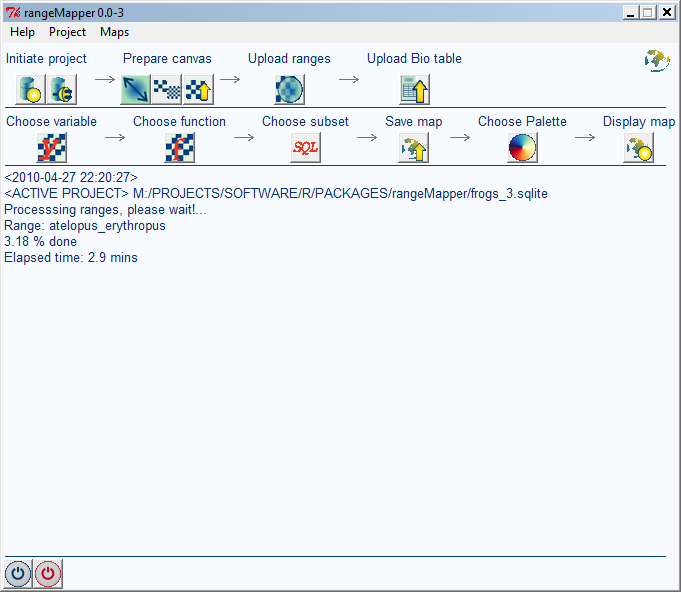
\includegraphics[width=1\linewidth]{fig1}
    \caption{\label{fig:fig1} \emph{rangeMapper} graphical user interface.}
  \end{center}
\end{figure}
To quickly get started, work through all the steps from \textit{Initiate project} to  \textit{Plot map} using the dataset and the range files which come together with the package (to find where they are located go to  \textit{ Help/Example files}). Place the mouse over each button to get tool-tips, (see fig. \ref{fig:fig2}). To get further help type  \texttt{?rangeMapper}  or \texttt{?} and the function name indicated by the tool-tip. 
	\begin{figure}[htbp]
	  \begin{center}
		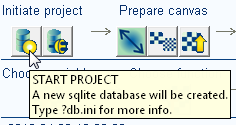
\includegraphics[width=0.5\linewidth]{fig2}
		\caption{\label{fig:fig2} Tool-tip example.}
	  \end{center}
	\end{figure}
 \pagebreak	
\section{rangeMapper step-by-step: project set-up}
	\subsection{Initiate/open project}
	\begin{figure}[htbp]
	  \begin{center}
		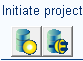
\includegraphics[width=0.2\linewidth]{fig3}
		\caption{\label{fig:fig3} Initiate project}
	  \end{center}
	\end{figure}
	At this step a new project is initiated by creating a new sqlite database and populating it with a few pre-formatted tables. 
	Type \texttt{?db.ini} for more details. You can stop at any of the next steps and resume latter by opening the same project.
	\\
	For the step-by-step tutorial, use the wrens dataset which is included within the package. This dataset contains the ranges and life history data on 45 species of wrens (Troglodytidae) \cite{ridgely07}. 
For more information on the dataset type at the R prompter:
\begin{Rcode}\begin{verbatim}
?wrens 
 wrens
\end{verbatim}\end{Rcode}
After pushing the initiate project button, choose a location to save the file, name your new project, for example `wrens', and press `OK'.

\subsection{Prepare canvas}
	
	\begin{figure}[htbp]
	  \begin{center}
		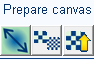
\includegraphics[width=0.2\linewidth]{fig4}
		\caption{\label{fig:fig4} Prepare canvas}
	  \end{center}
	\end{figure}
	
	Once the project has been initiated the next step is to prepare the canvas. 
	The canvas is a regular grid of a given resolution (in map units) defined
		for the rectangular area (i.e. the global bounding box) encompassing all the ranges. 
	
	At this step, (see fig. \ref{fig:fig4}) you have to:
	\begin{enumerate}
		 \item[-] Push the `COMPUTE CANVAS EXTENT' button and then select all the range polygon files (*.shp format) in order to define the global bounding box of the project. The global bounding box (see \texttt{?global.bbox} for more details) is computed using \texttt{getinfo.shape()} in \cite{maptools} package hence this step is reasonably fast even for thousands of range files. The vector (*.shp) files for the wrens ranges data are stored in the package's directory.  Access the `help/example files' menu to get the exact pathway for this directory.
		 \item[-] Push the `INPUT GRID SIZE' button and then input the desired resolution (a default value is provided). For the wrens, change the provided default of 125194.3m to a round 125000 m.
		 \item[-] "Push the `COMPUTE CANVAS' button to upload the canvas to the project's database.
	\end{enumerate}
	
	See \texttt{?canvas}  and \texttt{?sp::spsample} for more details.


	\subsection{Process and upload ranges}

	At this step you can select a directory containing the range files. Then every range polygon is overlaid on the canvas and the result of the overlap is saved to the database.\\
For the wrens, push the `PROCESS RANGES' button and select the directory with the wrens range vector files. Hit `YES' when asked to save range centroid and range extent data to the data project file.\\
Note that if there are thousands of range map polygons with complex geometries to be processed and/or the canvas resolution is relatively high this step can be time consuming. For example processing all amphibians of the world \cite{iucn09} (5816 ranges, total 252 MB) using a grid of 0.25$^{\circ}$ resolution takes 544 minutes on a 64-bit machine with 4 GB of RAM running Windows Vista and R 2.10.0. However, once this step has been performed and the results saved to the database, the other operations are fast.
	
	\subsection{ Upload external `BIO' data (e.g. life history data)}
	\begin{figure}[htbp]
	  \begin{center}
		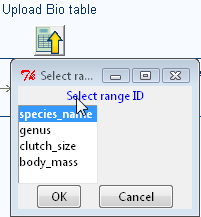
\includegraphics[width=0.5\linewidth]{fig6}
		\caption{\label{fig:fig6} Upload 'BIO' data}
	  \end{center}
	\end{figure}
	
If you are only  interested in species richness this step is optional. Data to be imported should be in .csv format (``;'' separated!). However, any \texttt{data.frame} can be imported from the command line. See \texttt{?rangeMapper} for an example and \texttt{?bio.save} for more details. During the importing of the `BIO' table you will be prompted to choose  the field, (see fig. \ref{fig:fig6}) corresponding to the range file names. The `BIO' table should thus contain a column with the file names of the range polygons (without the file extension). This column is used to link data in the `BIO' table to the range polygons data. \\ For the wrens example, push the `IMPORT BIO data' icon and select the `wrens.csv' data file stored in the package's directory (choose `Help/example' files to get the exact pathway to this file). Then select `species\_name' as the ID to link the data with the range files. You are now ready to draw some maps!

\section{rangeMapper step-by-step: drawing maps}		
	\subsection{ Choose a variable}
	
	\begin{figure}[htbp]
	  \begin{center}
		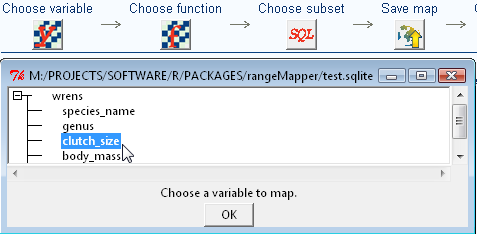
\includegraphics[width=0.9\linewidth]{fig7}
		\caption{\label{fig:fig7}Choose variable dialog}
	  \end{center}
	\end{figure}

	Once one or more `BIO' tables have been imported, the next step is choosing a variable (e.g. clutch size or body mass) to map, (see fig. \ref{fig:fig7}). For the wrens example, push the `CHOOSE VARIABLE' icon and select `clutch size'.
	
	\subsection{ Choose or define a function}
	\begin{figure}[htbp]
	  \begin{center}
		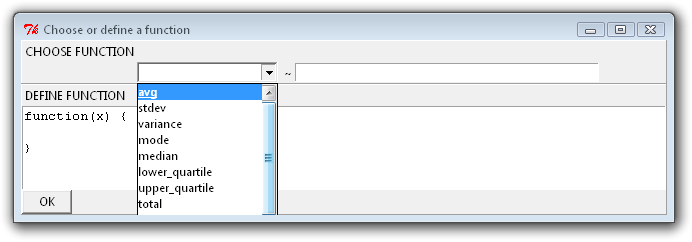
\includegraphics[width=0.9\linewidth]{fig8}
		\caption{\label{fig:fig8} Choose function dialog}
	  \end{center}
	\end{figure}
At this step you can choose or define a function to be applied at each canvas cell (see fig. \ref{fig:fig8}). For simple functions like \texttt{richness}, \texttt{mean}, \texttt{sd}, etc. or for a custom functions the formula is of form \texttt{response $\sim$ 1} (see \texttt{?lm} for more details on formula usage; and see section \ref{sec:wrensCV} for an example of a custom function used to calculate coefficient of variation). In the case of different models check \texttt{?assemblage.stat} for more details. \\
For the wrens example, push the `CHOOSE FUNCTION' icon and select `median'.
	
	
	\subsection{Choose subsets}
	\begin{figure}[htbp]
	  \begin{center}
		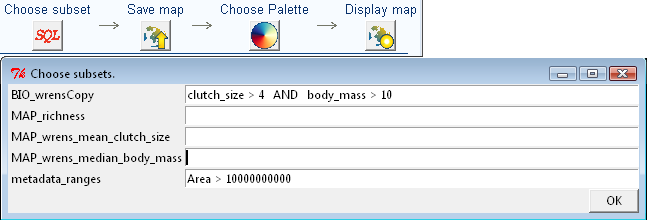
\includegraphics[width=1\linewidth]{fig9}
		\caption{\label{fig:fig9} Choose subsets}
	  \end{center}
	\end{figure}
At this step, (see fig.. \ref{fig:fig9}), you can select the data to be included in the `MAP', based on the field values of any of the existing `BIO', `MAP' or metadata\_ranges tables. The subset strings used in the `Choose subsets' dialog should be valid \texttt{WHERE} SQL clauses. Since this step is optional for the running wrens example, skip this step and go to on.
	
	\subsection{Save MAP}
	\begin{figure}[htbp]
	  \begin{center}
		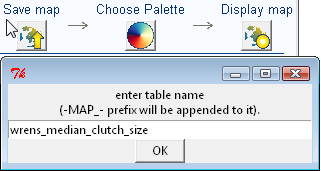
\includegraphics[width=0.5\linewidth]{fig10}
		\caption{\label{fig:fig10} Save MAP}
	  \end{center}
	\end{figure}

	At this step the program computes the previously chosen statistic (richness, average, median or any user-defined function) at each canvas cell and save the results to the database as a `MAP' table. For the wrens, push the `SAVE MAP' button, and name the map `median\_clutch' (see fig. \ref{fig:fig10}).
	
	
	\subsection{Choose a color palette}
	\begin{figure}[htbp]
	  \begin{center}
		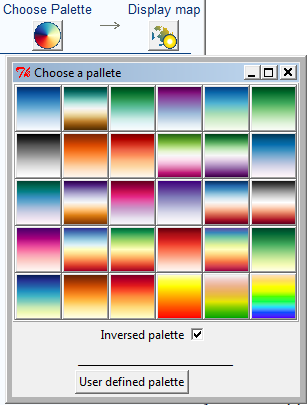
\includegraphics[width=0.5\linewidth]{fig11}
		\caption{\label{fig:fig11} Choose palette }
	  \end{center}
	\end{figure}

At this step you can  choose one of the available color palettes (see fig. \ref{fig:fig11}). There is the option to inverse the color palette if needed. Aditionally an a user defined palette can be constructed. See \texttt{?RColorBrewer::display.brewer.all} and \texttt{?colorRamp} for details and the underlying function used. For the wrens example, push the `CHOOSE PALETTE' button and select or build the palette you like.

	\subsection{Display a MAP}

Once a color palette is chosen, a map of the active project can be selected and displayed on the default graphic device (see fig. \ref{fig:fig12}). The number of grouping intervals and the class intervals type can be set here. For more info on class intervals see \cite{classInt} package. 
For the wrens, push the `DISPLAY MAP' button and accept the default value of 20 for the number of classes, and then select `equal' as the class interval type. Your map (see fig. \ref{fig:map2a}) should be ready on the default graphical device.

	
\begin{figure}
  \begin{center}
    \begin{tabular}{cc}
      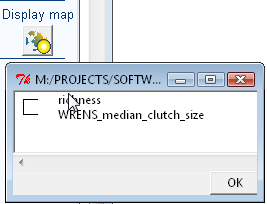
\includegraphics[width=0.5\linewidth]{fig12}
      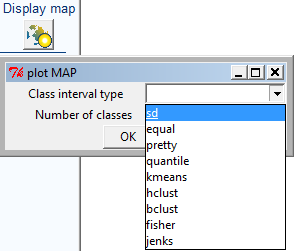
\includegraphics[width=0.5\linewidth]{fig13}
    \end{tabular}
    \caption{\label{fig:fig12} Display MAP}
  \end{center}
\end{figure}
	
\begin{figure}[htbp]
  \begin{center}
	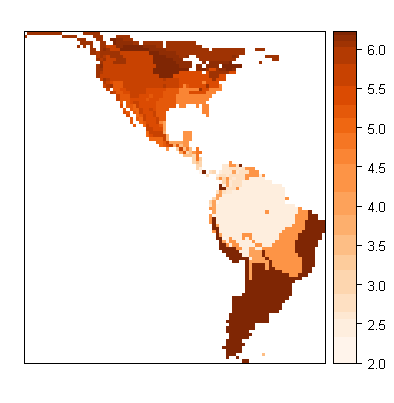
\includegraphics[width=0.5\linewidth]{map2a}
    \caption{\label{fig:map2a} Wrens: median clutch size}
  \end{center}
\end{figure}	
	
	
	\subsection{ More wren maps}
		\subsubsection{Wrens species richness}
Push the `CHOOSE FUNCTION' icon and select `richness'. Save the map, choose a new palette if you like, and display the new map (see fig. \ref{fig:map2c}). Note for species richness maps, it does not matter whether a specific variable is selected or not.
	
	\begin{figure}[htbp]
  \begin{center}
	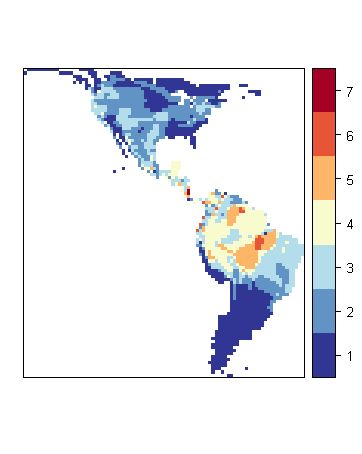
\includegraphics[width=0.5\linewidth]{map2c}
    \caption{\label{fig:map2c} Wrens: species richness}
  \end{center}
\end{figure}	
	
	
	\subsubsection{Wrens mean coefficient of variation  of body mass}
	\label{sec:wrensCV}

	Push the CHOOSE VARIABLE icon and select body mass. Then push the CHOOSE FUNCTION icon and type in the DEFINE FUNCTION BOX (between the curly brackets) the formula for coefficient of variation: "sd(x)/mean(x)" and then click OK. Save the map and display it (see fig. \ref{fig:map2b}).
	
	
		\begin{figure}[htbp]
  \begin{center}
	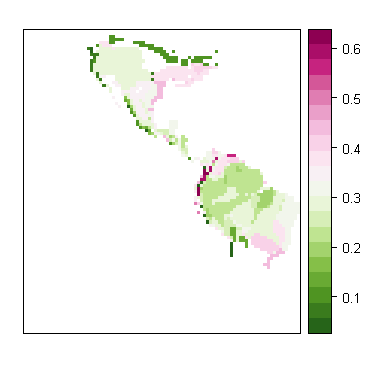
\includegraphics[width=0.5\linewidth]{map2b}
    \caption{\label{fig:map2b} Wrens: CV of body mass}
  \end{center}
\end{figure}	
	
\pagebreak		
\begin{thebibliography}{1}

\bibitem[sp]{sp}
	Pebesma, E.J., R.S. Bivand, 2005. Classes and methods for spatial data in R. R News 5 (2), 
			\url{http://cran.r-project.org/doc/Rnews/.}\\
	Roger S. Bivand, Edzer J. Pebesma, Virgilio Gomez-Rubio, 2008. Applied spatial data analysis with R. Springer, NY. 
			\url{http://www.asdar-book.org/}
			
\bibitem[maptools]{maptools}
	P Nicholas J. Lewin-Koh, Roger Bivand (2009). maptools: Tools for reading and handling spatial objects. R package version 0.7-29. \url{http://CRAN.R-project.org/package=maptools}			

\bibitem[rgdal]{rgdal}  
	Timothy H. Keitt, Roger Bivand, Edzer Pebesma and Barry Rowlingson (2010). rgdal: Bindings for the Geospatial Data
	Abstraction Library. R package version 0.6-25. \url{http://CRAN.R-project.org/package=rgdal }

\bibitem[sqlite]{sqlite}  
 David A. James (2010). RSQLite: SQLite interface for R. R package version 0.8-4. \url{http://CRAN.R-project.org/package=RSQLite}
  
\bibitem[Ridgely (2007)]{ridgely07}  
	 The breeding range files available in /extdata/wrens/vector/  package directory are available online at \url{http://www.natureserve.org/getData/dataSets/birdMapData/wrens.zip}. Data provided by NatureServe in collaboration with Robert Ridgely, James Zook, The Nature Conservancy - Migratory Bird Program, Conservation International - CABS, World Wildlife Fund - US, and Environment Canada - WILDSPACE.\\
Ridgely, R. S., T. F. Allnutt, T. Brooks, D. K. McNicol, D. W. Mehlman, B. E. Young, and J. R. Zook. 2007. Digital Distribution Maps of the Birds of the Western Hemisphere, version 3.0. NatureServe, Arlington, Virginia, USA.

\bibitem[classInt]{classInt}
Roger Bivand, with contributions by Hisaji Ono and Richard Dunlap (2009). classInt: Choose univariate class intervals. R package version 0.1-14. \url{http://CRAN.R-project.org/package=classInt}


\end{thebibliography}


\end{document}
	
	
	
	
	
	
	
	
	
	
	
	
	
	
	
	
	

	
